\documentclass[12pt]{article}
\usepackage{graphicx} % Required for inserting images
\usepackage[margin=1in]{geometry}
\usepackage{amsmath}
\usepackage{fancyhdr} % Required for custom headers/footers
%\usepackage{natbib} %useless and generates errors
%\bibliographystyle{unsrt} %useless and generates errors
\usepackage[backend=biber,style=numeric, citestyle=numeric-comp,sorting=none]{biblatex} %removing "backend=biber," does not affect the compilation process 
%style=ieee is not optimal
\addbibresource{biblio.bib}
%\bibliographystyle{ieeetr} %this does not work
% Customize the delimiter for supercites
\DeclareDelimFormat{multicitedelim}{\addcomma\space}
\usepackage{hyperref}
\usepackage{listings}
\usepackage{subfigure} %check in case of contrasts with other packages
\usepackage{float}
%\title{FMP_ Thesis}
%\author{Davide Biondi }
%\date{August 2024}

% Redefine the tableofcontents default name
\renewcommand{\contentsname}{Index of Contents}

\begin{document}
\newgeometry{top=2cm, bottom=1cm} % Adjust the top margin to 2 cm
\begin{titlepage}
\begin{center}

\begin{figure}
    \begin{center}
    
\includegraphics[scale=0.5]{unisa_logo.png}
    \end{center}   
\end{figure}
\begin{figure}
    \begin{center}
    
\includegraphics[scale=0.5]{uvic_logo_2.png}
    \end{center}
\end{figure}

\vspace*{-1cm}
\Large\textbf {Master of Science in Omics Data Analysis}
\vspace*{0.5cm}

\Large\textbf Master Thesis

\vspace*{0.5cm}

\huge\textbf{Human gut derived-organoids
provide model to study gluten
response and effects of microbiota
derived molecules in celiac disease}

\vspace{1cm}

\Large\textbf{Dr. Davide Biondi}
\vspace{1cm}


 
\begin{tabular}{@{}l@{\hspace{0.5cm}}l@{}}
Supervisor: & Prof. Roberto Tagliaferri, \\
            & DISA-MIS, University of Salerno (IT) \\
Tutor:      & Prof. Jordi Villà Freixa, \\
            & Departament de Biociències, \\
            & University of Vic (SP) \\
\end{tabular}


\vspace{1cm}

\large{Biosciences Department}


\vspace{0.5cm}

\large{University of Vic – Central University of Catalonia}

\vspace{0.5cm}

\large{\today}

\end{center}
\end{titlepage}
\restoregeometry

% Set up fancy page style for pages after the title page
\fancypagestyle{myfancy}{
    \fancyhf{} % Clear all header and footer fields
    \fancyfoot[C]{\thepage} % Place page number at center of the footer
    \renewcommand{\headrulewidth}{0pt} % Remove header line
    \renewcommand{\footrulewidth}{0pt} % Remove footer line
}

% Apply the custom page style
\pagestyle{myfancy}

\newgeometry{top=2cm} % Adjust the top margin to 1cm
\tableofcontents  % Add the section

\restoregeometry

\section{Summary}
% Begin the paragraph with a larger font size and bold text
% Redefine paragraph to use large and bold
% Use \leavevmode to ensure proper spacing
\paragraph{\large \textbf{Abstract}}\mbox{} \\

\noindent Celiac disease (CD) is an immune-mediated condition triggered by exposure to gluten. Although extensive research has been conducted on the role of the adaptive immune system in CD development, a lack of effective experimental models has limited our insight into the initial stages that lead to gluten intolerance. By utilizing intestinal organoids derived from duodenal biopsies of both non-celiac (NC) and celiac (CD) patients, I investigated the role of the gut epithelium in CD pathogenesis, focusing on how the epithelium responds to gluten. Compared to NC organoids, RNA sequencing of CD organoids demonstrated significant changes in the expression of genes related to the gut barrier and innate immune response. A total of 83 differentially expressed genes has been discovered, of which 45 were overexpressed in CD patients, and 38 were underexpressed.
\paragraph{\large \textbf{Abbreviations}}\mbox{} \\

\noindent CD = Celiac disease
NC = Non-celiac ; SE = Single-end ; PE = Paired-end ; GSEA = Gene Set Enrichment Analysis ; GOA = GO annotation analysis ; GFD = Gluten-free diet ; GCD = Gluten-containing diet ; 
DAVID = Database for Annotation, Visualization and Integrated Discovery ; STAR = Spliced Transcripts Alignment to a Reference ; 
TEER = Transepithelial electrical resistance ; PDTOs = Patient-derived tumor organoids ; iPSCs = Induced pluripotent stem cells ; 
TG2 = Transglutaminase 2 ; tTG = Tissue transglutaminase ; HLA = Human leukocyte antigen ; HP = Haptoglobin ; ReA = Reactive arthritis ; RA = Rheumatoid arthritis ; ACPA = Anti-citrullinated protein antibodies ; IFN = Interferon ; IL = Interleukin ; 
EGFR = Epidermal growth factor receptor ; TGF = Transforming growth factor ; Th = T helper cells ; 
SARA = SMAD anchor for receptor activation ; HMMs = Hidden Markov Models ; SAs = Suffix arrays ; 
PTPRK = Protein Tyrosine Phosphatase Receptor Type K ; DEFA6 = Defensin, alpha 6 ; HD6 = Human alpha defensin 6 ; 
TSP-1 = Thrombospondin-1 ; GPIV = Glycoprotein IV ; HVR = Hypervariable region ; SEP = shared epitope

\section{Introduction}
\noindent 3D cell culture models, such as spheroids and organoids,
were developed to better mimic the spatial and microenvironmental information of the in vivo situation. Organoids can be established from embryonic stem cells, adult stem cells, or induced pluripotent stem cells (iPSCs) \supercite{kim2020comparison}. Patient-
derived tumor organoids (PDTOs) can be grown directly from patient tissue biopsies or surgically removed tumor tissues, the same applies for duodenal biopsies of NC and CD patients. Organoids can form organ-like structures reminiscent of the tissues they originated from and contain both stem and differentiated cell populations resembling patient tissues. Histological characteristics, such as crypt hyperplasia and villous blunting, are defining features of active celiac disease (CD). This condition is marked by an increase in the population of immature cells, accompanied by a simultaneous decrease in the mature cells of the villi. \supercite{piscaglia2015circulating}. These pathological changes in the intestinal mucosa associated with CD are believed to result from a defective stem cell compartment that fails to adequately support tissue regeneration and/or from heightened epithelial apoptosis \supercite{shalimar2013mechanism}. A study highlighted the role of inflammation in CD, noting that even in the absence of gluten, there is a low-grade inflammation present in CD cells and organoids. This suggests that organoids can be a valuable tool for studying the inflammatory processes in CD, even before gluten exposure \supercite{barone2022pivotal}. Another study suggested that the inflammatory markers pNF-$\kappa$B, pERK,
IL-1$\beta$, and IL-6 were increased and persistent in CD organoids \supercite{porpora2022inflammation}.
Celiac disease is also considered a "Western" pathology, because in general, the Western diet and lifestyle have been long linked to low-grade inflammation that represents the “common background” of
several different diseases \supercite{minihane2015low}. Celiac disease is an immune-mediated enteropathy triggered in genetically susceptible individuals
by a group of wheat proteins and related prolamins from cereals \supercite{sollid2013triggers}. It is induced by gluten consumption in individuals genetically predisposed with HLA-DQ2 or HLA-DQ8 haplotypes \supercite{leonard2017celiac}.
As regarding the molecular pathology aspect of the disease, we know that the enzyme transglutaminase 2 (TG2) plays a key role in celiac disease (CD) pathogenesis. Active TG2 is located mainly extracellularly in the lamina propria but also in the villous enterocytes of the duodenum. The TG2 inhibitor ZED1227 is a promising drug candidate for treating CD and is designed to block the TG2-catalyzed deamidation and crosslinking of gliadin peptides \supercite{isola2023oral}. This role of TG2 has as a consequence the proliferation of gluten-specific and tissue transglutaminase (tTG) antibodies expressed during the acute phase \supercite{husby2012european}.
Another pivotal role in the pathogenesis of CD is played by the
HLA (human leukocyte antigen)-restricted gliadin-specific intestinal T cell response \supercite{sollid2013triggers,iversen2020evidence}.
Although activation of T cells has been studied in depth, the central question still remains
unanswered, namely, why a pro-inflammatory T cell response is generated toward gliadin
instead of a regulatory response, which normally promotes oral tolerance to dietary protein
antigens. When, how and where this inflammation is generated in CD is not clear.
The evaluation of the haptoglobin (HP) genotype of the organoids employed in the study is also important. Haptoglobin encodes for two alleles, of which HP2 carries a duplication of the 3$^{\text{rd}}$ and 4$^{\text{th}}$ exons \supercite{maeda1984duplication}. The allele HP2, encodes for the HP2 pre-haptoglobin also known as zonulin, that has been shown to be a physiological regulator of tight junctions and it is released upon gluten stimulation \supercite{lammers2008gliadin}. All the organoids in this study had at least one copy of the HP2 allele (HP2-1 or HP2-2 genotype). Based on available evidence, it is suggested that the onset of CD follows this sequence of events: after ingestion, undigested gliadin peptides stimulate the release of zonulin, resulting in increased intestinal permeability \supercite{drago2006gliadin,hollon2015effect}. The compromised barrier permits the translocation of gliadin peptides into the lamina propria, where they interact with macrophages and other immune cells \supercite{fasano2011zonulin}. Gliadin peptides trigger IL8 and IL15 secretion from enterocytes, which in turn recruits neutrophils \supercite{lammers2011identification} and intraepithelial lymphocytes \supercite{di2006epithelium}. Ultimately, the engagement of T cells with cells presenting gliadin peptides in a pro-inflammatory environment results in the breakdown of oral tolerance and the activation of the Th1/Th17 adaptive immune response \supercite{serena2015role}. In this study we focused on spotting the aforementioned genes in our differentially expression analysis, based on the hypothesis that organoids can reproduce the epression patterns of CD patients.

 
\section{Materials and Methods}
\paragraph{Hardware specs influence on results}\hspace{0pt}\\\\
\noindent Most of the pre-processing (till the rRNA sequence removal) has been done on a Linux Mint machine, with the following system specifications:
System:    Kernel: 5.4.0-135-generic x86\_64 bits: 64 compiler: gcc v: 9.4.0 
           Desktop: Cinnamon 4.6.7 wm: muffin dm: LightDM Distro: Linux Mint 20 Ulyana 
           base: Ubuntu 20.04 focal 
Machine:   Type: Laptop System: Dynabook product: SATELLITE PRO C50-E-10R v: PYS20E-00L0D2IT 
           
           Mobo: Dynabook model: DBIIP300  
           UEFI: American Megatrends v: KN16RV100 
           date: 05/26/2020 
CPU:       
Topology: Dual Core model: Intel Core i3-8130U bits: 64 type: MT MCP arch: Kaby Lake 
           rev: A L2 cache: 4096 KiB 
           flags: avx avx2 lm nx pae sse sse2 sse3 sse4\_1 sse4\_2 ssse3 vmx bogomips: 17599 

These specs were obtained with the bash command inxi.
The rest of the RNA-seq pipeline from indexing of the genome, reads mapping and quantification till GSEA was done on an Ubuntu machine with the following system specifications:
System:
  Kernel: 5.15.0-119-generic x86\_64 bits: 64 compiler: N/A 
  Desktop: Gnome 3.36.9 wm: gnome-shell dm: GDM3 
  Distro: Ubuntu 20.04.6 LTS (Focal Fossa) 
Machine:
  Type: Desktop System: Dell product: Precision Tower 5810 v: N/A 
  Chassis: type: 7  
  Mobo: Dell model: 0HHV7N v: A00 
  UEFI: Dell v: A20 
  date: 07/26/2017 
CPU:
  Topology: 10-Core model: Intel Xeon E5-2630 v4 bits: 64 type: MT MCP 
  arch: Broadwell rev: 1 L2 cache: 25.0 MiB 
  flags: avx avx2 lm nx pae sse sse2 sse3 sse4\_1 sse4\_2 ssse3 vmx 
  bogomips: 87798 
  

\noindent Addressing not only the software specifications, but also the hardware ones, is important, because a computer hardware architecture can have an impact not only on the time required to execute a certain algorithm, but on the output itself. This is true when it comes to floating-point arithmetic \supercite{goldberg1991every}. Floating-point representations have a base $\beta$, (which is always assumed to be even) and a precision $p$. If $\beta=10$ and $p=3$, the number 0.1 is represented as $1.00\times10^{-1}$. 
\paragraph{Adapter sequence trimming and QC}\hspace{0pt}\\\\
The RNA-seq data in fastq format was downloaded from the GEO database \supercite{samples}. From the downloaded data all the Phred scores for all the bases resulted as leveled to 30 (assigned with the symbol "?"). The real raw SRA data were not available due to unidentified issues. Nonetheless, quality control was completed using trim-galore version 0.6.10 build hdfd78af\_0, installed from Bioconda channel. The conda virtual environment in which Trim Galore was launched had Python version 3.8.19, and cutadapt 4.9. The adapter sequence was AGATCGGAAGAGC. The trimming mode was for single-end reads. The cutoff for removing sequences was 20 bp. The quality Phred score cutoff was set up as 20. Trim Galore uses Cutadapt to identify and remove adapter sequences from the 3' end of reads. By default, it trims the first 13 base pairs of standard Illumina adapters. The tool trims low-quality bases from the 3' end of reads, as mentione before. This is done before adapter trimming to ensure that only high-quality data is retained for downstream analysis \supercite{trim_galore}. After trimming, reads that are shorter than a specified length can be removed in a length filtering, to prevent issues during alignment and analysis. FastQC  was used after trimming the adapter sequences, as it is considered a best practice. FastQC - which is used together with Cutadapt with Trim Galore acting as a wrapper between the two - performs a series of modular analyses, each focusing on different aspects of the data quality. These analyses include:
Per Base Sequence Quality: Assesses the quality scores across all bases at each position in the reads. It helps identify regions with low-quality scores that may need trimming.
Per Sequence Quality Scores: Evaluates the distribution of quality scores across all reads to detect any reads with universally low quality.
Per Base Sequence Content: Analyzes the proportion of each nucleotide at every position in the reads. Imbalances may indicate biases or contamination.
Per Sequence GC Content: Provides a density plot of the GC content across all reads, which can highlight unusual patterns.
Overrepresented Sequences: Identifies sequences that occur more frequently than expected, which may indicate contamination or adapter sequences.
Adapter Content: Detects the presence of adapter sequences within the reads. 
K-mer Content: Analyzes the frequency of short nucleotide sequences (k-mers) to identify biases \supercite{fastqc}. 
\paragraph{rRNA sequences removal}\hspace{0pt}\\\\
After this initial trimming/quality-control step, rRNA sequences removal has been executed with sortmerna version 4.3.6 build h9ee0642\_0 installed through bioconda channel. SortMeRNA utilizes a seeding strategy that focuses on identifying short regions of similarity between rRNA sequences in a database and the input reads. This approach is akin to the use of Hidden Markov Models (HMMs) but is executed significantly faster \supercite{kopylova2012sortmerna}. SortMeRNA uses a burst tries data structure coupled with a lookup table to efficiently store and access the rRNA database. This setup enhances the speed and accuracy of the filtering process \supercite{kopylova2012sortmerna}. The filtering was ran using default parameters, namely seed length as 18, Gumbel lambda as 0.601061, Gumbel K as 0.328323. The other parameters are available in the GitHub \supercite{github}. 
\paragraph{Genome indexing and reads mapping}\hspace{0pt}\\\\
After indexing the hg19 fasta file genome from UCSC genome browser, using a GTF ENSEMBL annotation file from the same portal, the mapping of the reads without rRNA was done. Indexing and mapping were performed using star version 2.5.2b build 0 from bioconda channel. Mapping consists of two phases: seed finding, and then another phase of clustering, stitching and scoring. Seed finding phase is the sequential search for a Maximal Mappable Prefix (MMP) \supercite{dobin2013star}. 
The splice junctions are detected in a
single alignment pass without any a priori knowledge of splice
junctions’ loci or properties, and without a preliminary contiguous alignment pass needed by the junction database approaches \supercite{dobin2013star}. 
The MMP in STAR search is implemented through uncompressed suffix arrays (SAs) \supercite{manber1993suffix}. Finding MMP is an inherent outcome of the standard binary string search in uncompressed SAs. The MMP search, implemented in STAR, enables finding multiple mismatches and indels. If the MMP search does
not reach the end of a read because of the presence of one or
more mismatches, the MMPs will serve as anchors in the genome
that can be extended, allowing for alignments with mismatches.
In some cases, the extension procedure does not yield a good
genomic alignment, which allows identification of poly-A tails,
library adapter sequences or poor sequencing quality tails \supercite{dobin2013star}.
In the second phase of the algorithm, STAR builds alignments of the entire read sequence by stitching together all the seeds that were aligned to the genome in the first phase. First, the seeds are clustered together by proximity to a selected set of ‘anchor’ seeds \supercite{dobin2013star}. 
All the seeds that map within user-defined genomic windows
around the anchors are stitched together assuming a local linear
transcription model. The stitching is guided by a local alignment scoring scheme, with user-defined scores (penalties) for matches, mismatches, insertions, deletions and splice junction gaps, allowing for a quantitative assessment of the alignment qualities and ranks \supercite{dobin2013star}. 
STAR was set up for both reads mapping and quantification, in order to have additional control of the quantification step so that reads counts could be compared between STAR and HTseq. The reads average length was 50, so it got diminished of one unit in the STAR parameters, as suggested by the developers. SAM files were also generated during the operations with STAR, as diagnostic tools, and as a best practice. The BAM files generated with STAR and accepted from HTseq as input were of the type "SortedByCoordinate".
STAR does not need to know the strandness of the data, but the strandness of the reads and their length are fundamental parameters in both indexing of the genome, and mapping and quantification of the reads. A bash script was used in order to assess the strandness of the reads, parsing "out.tab" files obtained as output from STAR reads mapping and quantification, and another script was used in order to check the average length of the reads by parsing the fastq files with awk text processing tool.
\paragraph{Quantification}\hspace{0pt}\\\\
\noindent The quantification (read counts over transcripts) which was used for downstream analysis was completed 
with HTseq version 0.6.0 \supercite{anders2015htseq}. Quantification was ran with the basic default parameters.
Again, HTseq parameters had to mirror the ones used for STAR, so a parameter was set up for HTseq to recognize reads on the reverse strand, where the reads selectively map; regarding the key --nonunique parameter, this is by default set as "none", so the read (or read pair) is counted as ambiguous and not counted for any features. Also, if the read (or read pair) aligns to more than one location in the reference, it is scored as alignment\_not\_unique \supercite{htseq_docs}. Another parameter was set up in order to address the kind of file to parse, in this case BAM sortedByAlignment, as mentioned before. 
\paragraph{Downstream analysis}\hspace{0pt}\\

\noindent Differential 
expression analysis on the read counts over transcripts was conducted with pydeseq2 \supercite{muzellec2023pydeseq2} version 0.4.4 build 
pyhdfd78af\_0 from bioconda channel. Genes with a total of less than 10 counts were excluded, and after this filtering, genes with baseMean $>=$ 
10, of which adjusted p value $<$ 0.05 and absolute value of log2FC $>$ 0.5 
were selected as differentially expressed genes. Functional gene set enrichment analysis (GSEA) was performed on the whole-
transcriptome expression values using gseapy \supercite{fang2023gseapy} 
version 1.1.3 build py38he1d39cf\_1 from bioconda channel, with a comparison against 'GO Biological Process 2021' gene sets with default 
parameters. Functional annotation analysis was performed on differentially expressed genes using DAVID v6.8 \supercite{huang2007david,huang2007david_2}. Gene set enrichment analysis is ran on the whole-transcriptome expression values compared to GO annotation analysis (GOA), because it can capture subtle changes between the samples conditions that GOA could miss. It is done in conjunction with GOA as a best practice in order to get the biological meaning of the data as a whole.

 
\section{Results}
\noindent During the pre-processing with Trim Galore the sequences removed because they became shorter than the length cutoff were between the 0.3-0.5\%. The fastqc report signaled warnings regarding the sequence duplication levels, and the per base sequence content, that would be difficult to address without a precise protocol followed by the authors for the PCR and the library preparation.
The results of the filtering with SortMeRNA pointed out that between 99,97\% and 99,98\% of the reads failed the E-value threshold, meaning that they do not contain rRNA.
The output of STAR concerning reads mapping and quantification consisted in a range of 16–21 million aligned single-end 50 bp reads per sample, mapped on the reverse strand. This is because the majority of the library preparation protocols are designed to produce stranded reads, most of the time mapping on the reverse strand.

\noindent Out of the most interesting DEGs found during the differential expression analysis (DEA), DKK1, a WNT negative regulator \supercite{fedi1999isolation} was significantly down-regulated. Trefoil factors (TFF1 and TFF2) were also significantly down-regulated. Trefoil factors (TFFs) are a family of small peptides that play crucial roles in maintaining and repairing mucosal surfaces, particularly in the gastrointestinal tract. On the other hand, the upregulation of NLRP6, initiator of the inflammasome
complex formation \supercite{levy2017nlrp6}, has been confirmed. Another gene confirmed as overexpressed is Defensin, alpha 6 (DEFA6) also known as human alpha defensin 6 (HD6). 
\begin{figure}[htb] %[htb] is important to force image positioning
    \centering
    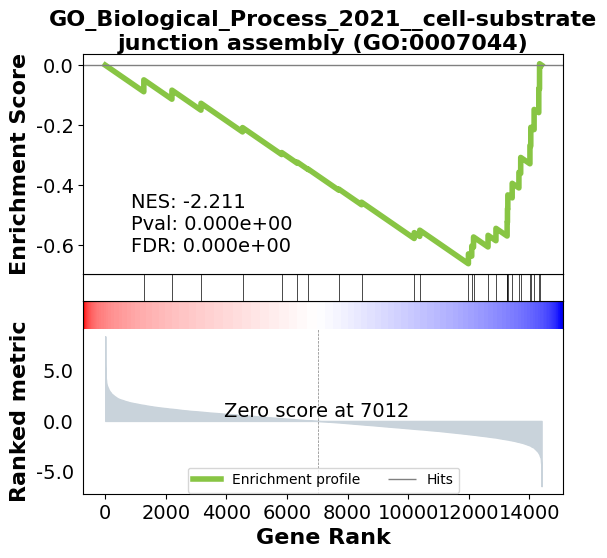
\includegraphics[width=0.55\textwidth]{gseaplot_2.png}
    \caption{GSEA plot showing the most significant negative normalized enrichment score (NES), considering its absolute value was the highest. The gene set for the term "cell-substrate junction assembly" is more associated with the control group than with the disease group.The red area indicates genes that are more prevalent in the disease group, while the blue area shows those more prevalent in the control group. This means that most of the genes in this set are highly expressed or prevalent in the control samples compared to the disease samples }
\end{figure}
 
\noindent One interesting finding is the overexpression of CD36, a membrane protein that belongs to the class B scavenger receptor family. In cancer, CD36 expression promotes tumor development,
metastasis, drug resistance \supercite{guerrero2022role}. Also known as platelet glycoprotein IV (GPIV), it was demonstrated to be a receptor for thrombospondin-1 (TSP-1), a glycoprotein involved in platelet adhesion and an endogenous inhibitor of angiogenesis \supercite{feng2023role}.
\begin{figure}[H] % Use [H] to enforce placement
    \centering
    
        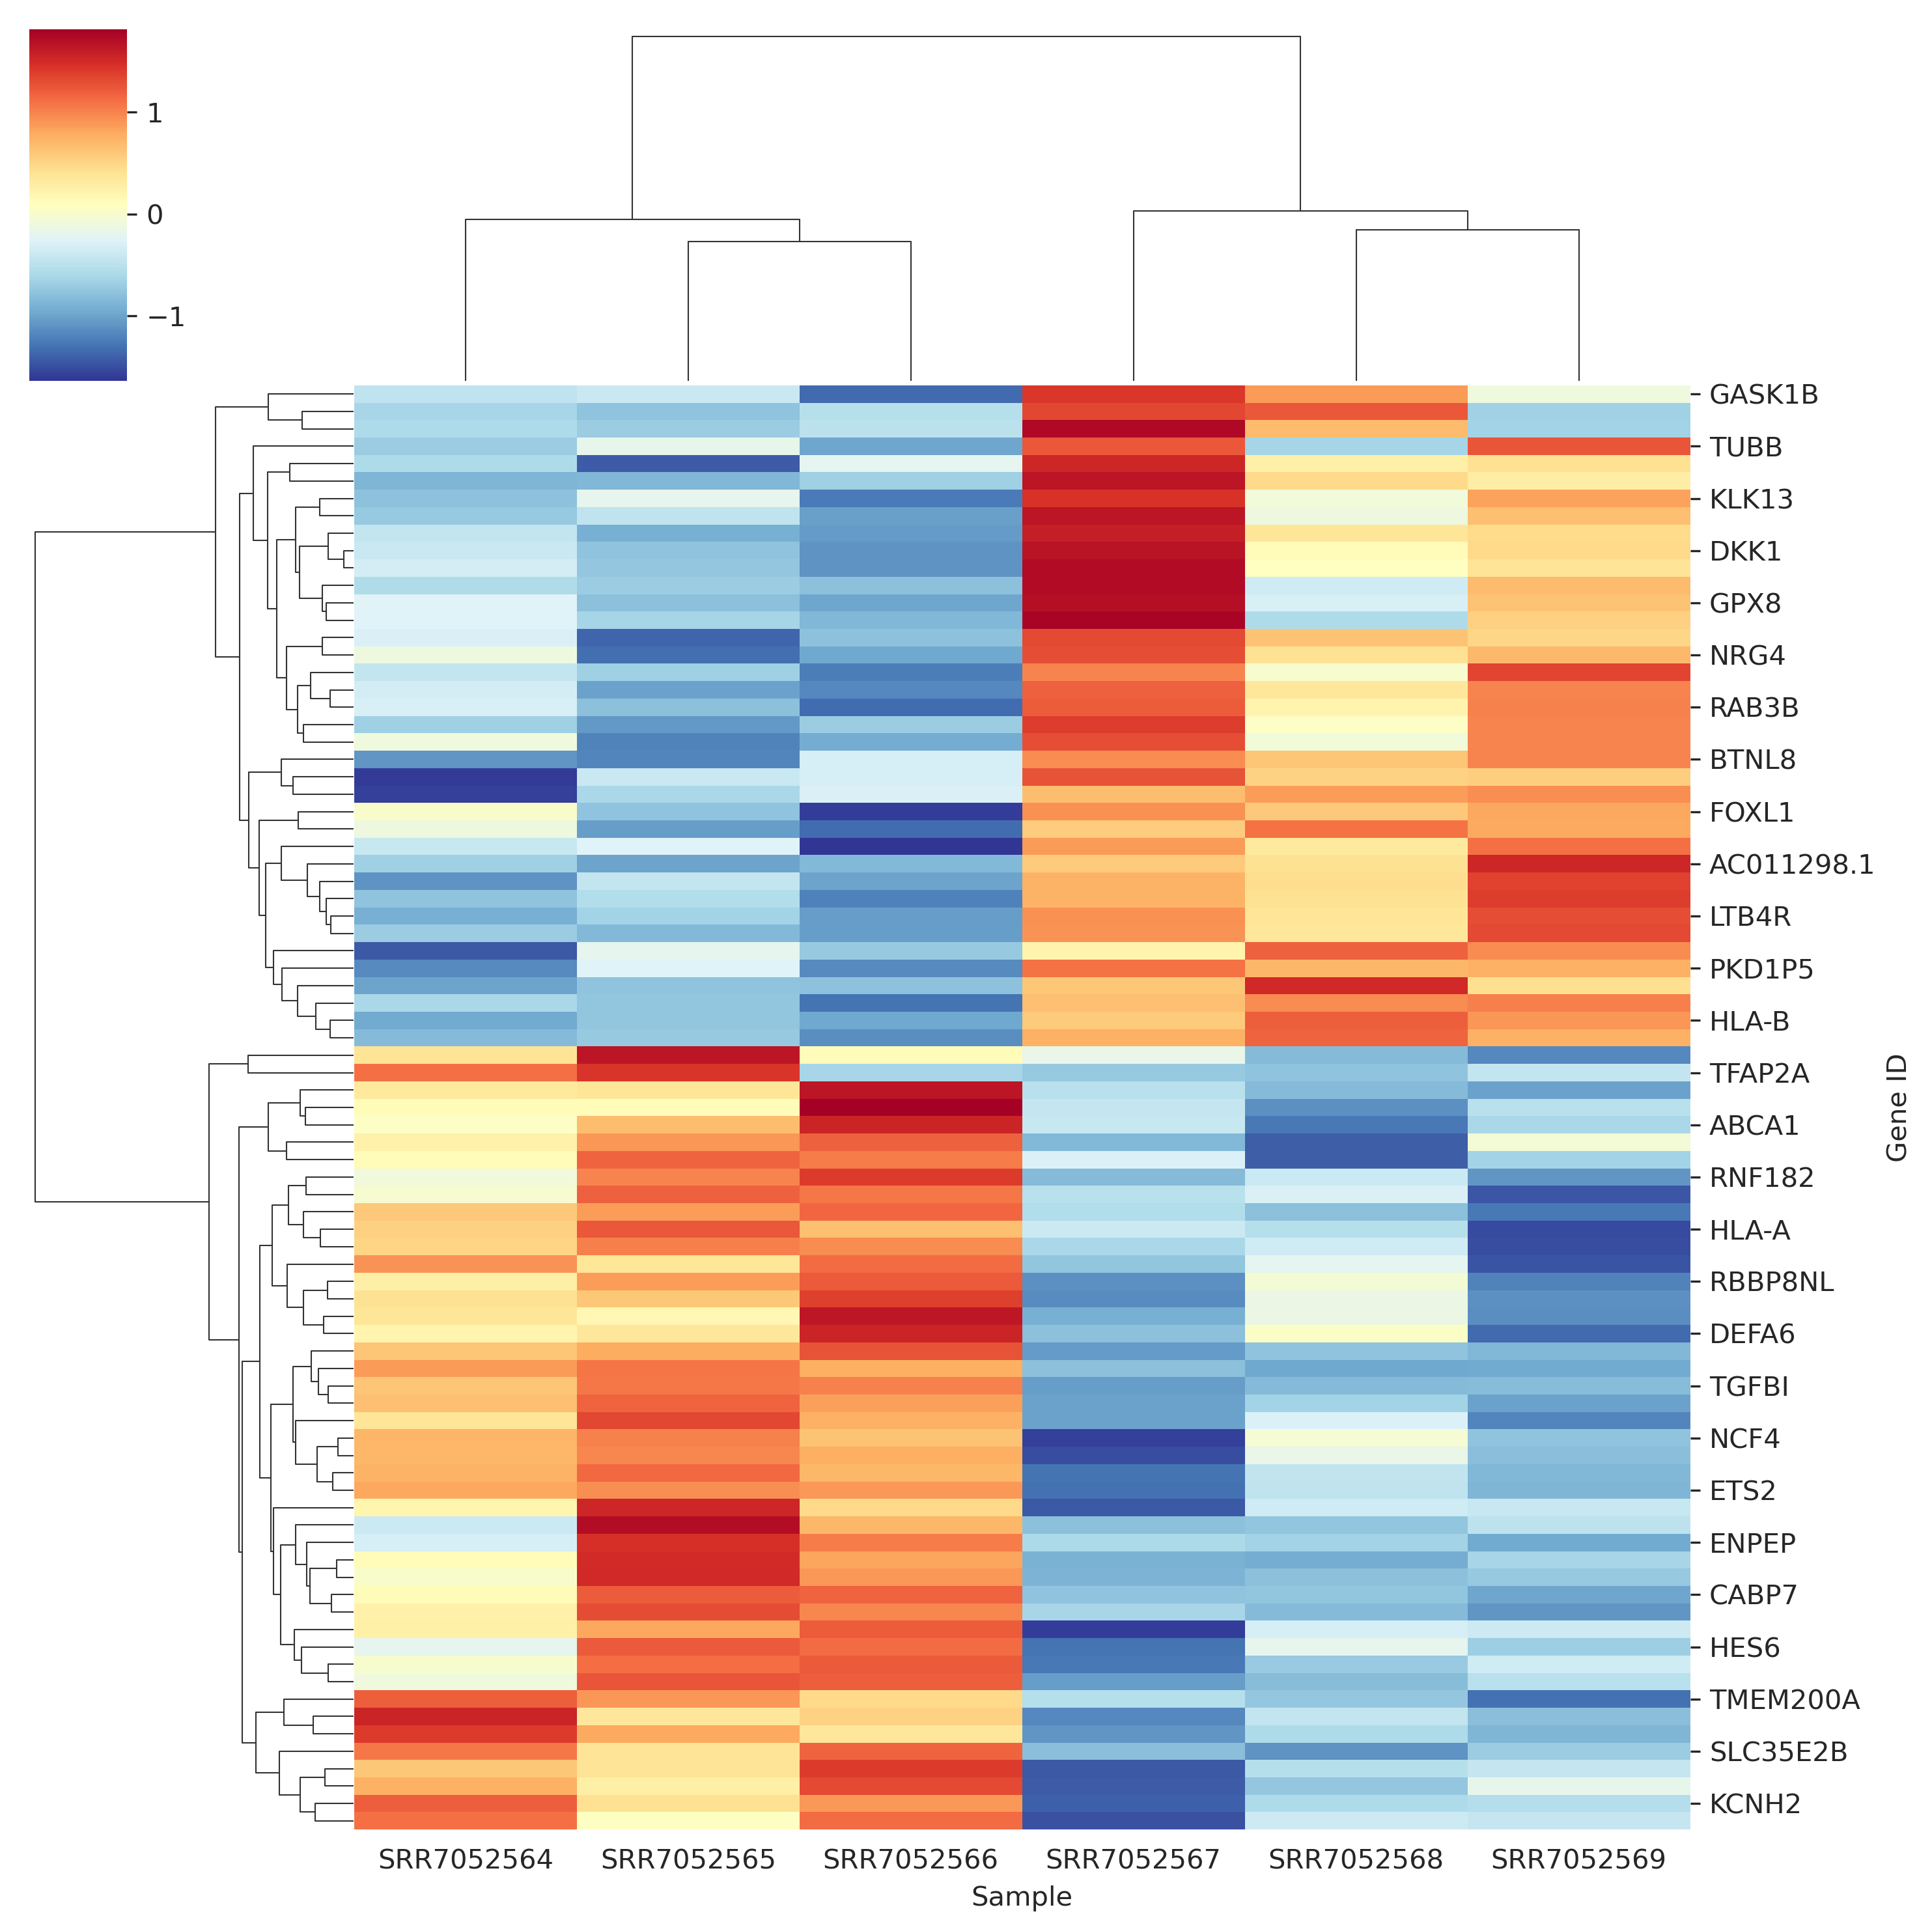
\includegraphics[width=0.55\textwidth]{clustermap_symbols_quant_4.png}
        \label{fig:Heat map}
        \caption{Heatmap representing RNA-seq expression values for the genes differentially
expressed in organoids from patients with active celiac disease (CD, n = 3) compared to non-celiac controls (NC, n = 3). A color code from blue to red indicates low and high expression levels, respectively.}
\end{figure}    
\noindent Interesting is also the overexpression of TGFBI with a high level of significance, and it has been suggested that the role of TGF-$\beta$ in Th17 differentiation is the suppression of Th1 and Th2 differentiation (i.e. suppression of the production of IFN-$\gamma$ and IL-4), since these cyokines strongly inhibit Th17 differentiation, but according to a report, ROR$\gamma$t, the master regulator of Th17, was induced by TGF-$\beta$ alone even in the absence of IL-6 \supercite{ichiyama2008foxp3}.
\begin{figure}[H]
    \centering
        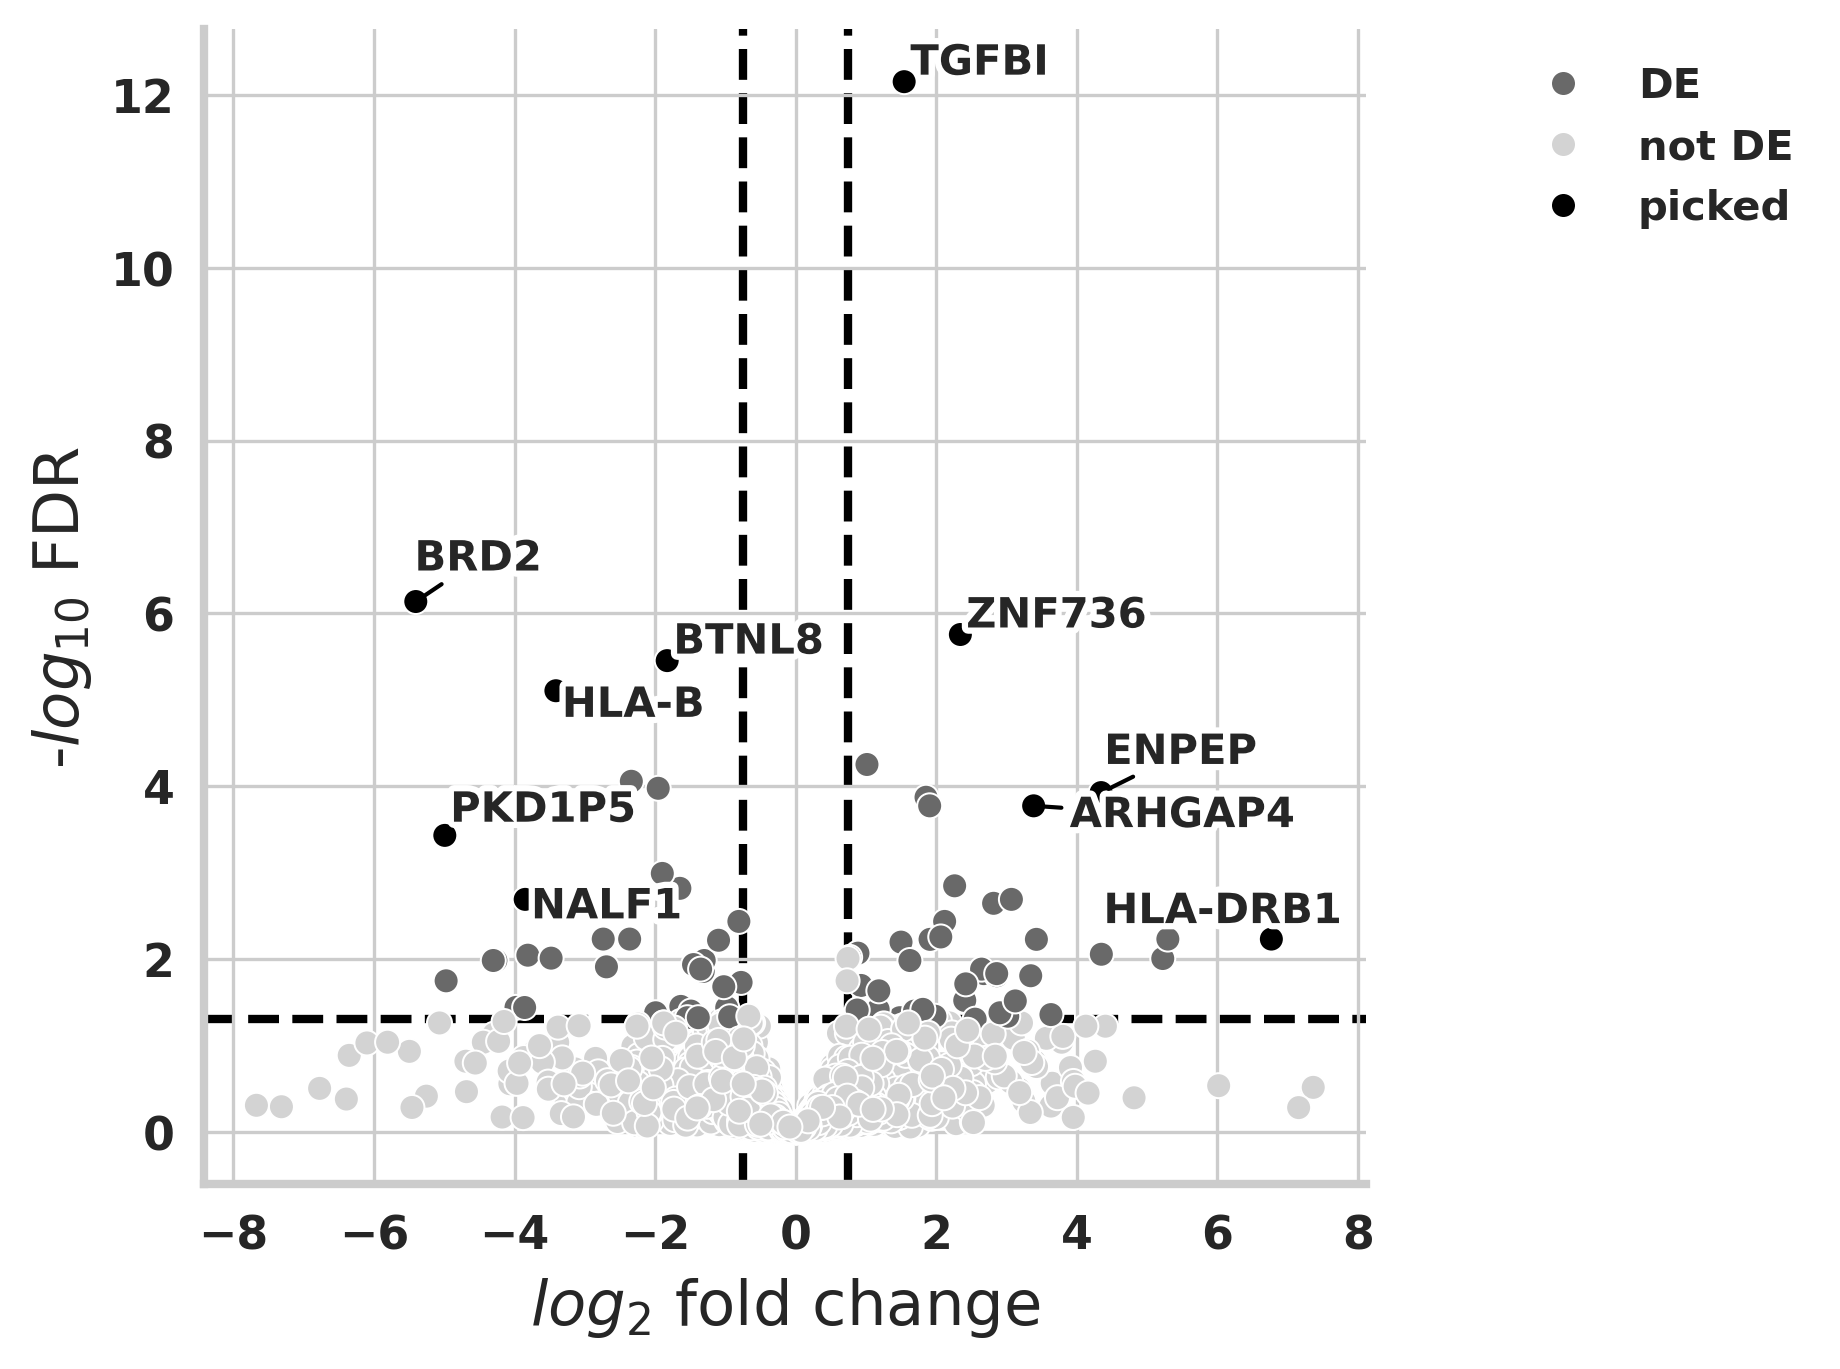
\includegraphics[width=0.55\textwidth]{volcano_plot_quant_4.png}
        \label{fig:Volcano plot}
    
    \caption{Volcano
plot showing fold change (X axis in $log_{2}$ scale) and statistical significance (FDR, Y axis in $-log_{10}$ scale) for
differentially expressed genes (RNA-seq) in active celiac (CD, n = 3) compared to non-celiac (n = 3) organoids}
    \label{fig:Volvano plot}
\end{figure}
\noindent Another suspect and overexpressed gene, visible in the volcano plot, is HLA-DRB1. HLA-DRB1 gene alleles are often linked to these celiac-associated HLA-DQ aplotypes such as HLA-DQ2 and HLA-DQ8. In a report on tens of Lybian children suffering both CD and type 1 diabetes mellitus, 70\% carried the HLA-DQ2 linkage with
HLA-DRB1 alleles \supercite{ghawil2012hla}. Human leukocyte antigen (HLA) region is located on chromosome 6. The region
consists of genes encoding molecules responsible for regulating immune response. HLA molecules are cell surface–bound glycoproteins classified into three classes. HLA class II is expressed on the surface of antigen-presenting cells (including macrophages, B cells and dendritic cells)
and is essential in order to display peptides to T-helper CD4$+$ cells, inducing their activation. HLA class
II antigens are mainly encoded by DR, DQ \supercite{wysocki2020current}.


\section{Discussion}
TFF1 contributes to the protection of the gastric mucosa by enhancing the stability and viscosity of the mucous layer, which acts as a barrier against gastric acid and pathogens \supercite{braga2020structure}. TFF2, also known as spasmolytic polypeptide, is predominantly found in the stomach, secreted by the mucous neck cells. TFF2 plays a significant role in protecting the gastric lining and aiding in its repair after injury. It is involved in maintaining the integrity of the mucosal barrier and supports epithelial restitution \supercite{aihara2017trefoil}.TFF2 is expressed in immune cells and has been implicated in modulating immune responses, particularly in the context of gastrointestinal inflammation \supercite{hoffmann2021trefoil}; in addition to that, it forms complexes with mucin MUC6, contributing to the stabilization of the inner layer of gastric mucus, which is crucial for protecting the stomach lining from digestive enzymes and pathogens \supercite{hoffmann2021trefoil}. Defensin, alpha 6 (DEFA6) also known as human alpha defensin 6 (HD6) affords protection against invasion by enteric bacterial pathogens by self-assembly to form fibrils and nanonets that surround and entangle bacteria \supercite{chu2012human}. NLRP6, initiator of the inflammasome
complex formation is overexpressed, as mentioned before. In celiac disease, the NLRP6 inflammasome is expressed in intestinal epithelial cells. This expression is associated with the production of caspase-1 and biologically active interleukin-18, which can further induce interferon-$\gamma$ in intraepithelial lymphocytes
\supercite{pietz2017immunopathology}, potentially exacerbating inflammation and tissue damage. Intestinal epithelial cells (IECs) produce inflammasome cytokines in response to noxious agents and selected microorganisms. The inflammasome cytokine IL-18, also known as
IFN-$\gamma$-inducing factor, is most likely the inducer. It is expressed at very high levels in IECs in
active CD \supercite{pietz2017immunopathology}. PTPRK transcription is directly regulated by TGF-$\beta$ through binding of Smad3/4 to the proximal promoter region of the PTPRK gene, so TGF-$\beta$ induce PTPRK gene expression \supercite{xu2015notch}. And one of the roles of PTPRK (Protein Tyrosine Phosphatase Receptor
Type K), a nodal phosphatase is the regulation of EGFR activation in the proliferation of the
enterocytes from CD biopsies and organoids. The overexpression of PTPRK in CD organoids is able to reduce pEGFR, pERK and proliferation. The activation of the EGFR/ERK pathway is linked to increased proliferation of enterocytes \supercite{nanayakkara2022ptprk}. This pathway is crucial in CD, where enterocyte proliferation is dysregulated, leading to crypt hyperplasia and villous atrophy. TGF-$\beta$s signal via a pair of transmembrane serine/threonine protein kinases, known as the type I (TGF-$\beta$R1 or ALK5) and type II receptors (TGF-$\beta$R2). Binding of one of these cytokines to a TGF-$\beta$R2 dimer triggers the recruitment and subsequent transphosphorylation of TGF-$\beta$R1 which, in turn, activates the downstream canonical signaling cascade via the receptor-regulated SMADs (R-SMADs). Upon receptor activation, phosphorylation of SMADs causes their dissociation from SARA (anchor for receptor activation) and formation of SMAD2/3–SMAD4 complexes \supercite{tsukazaki1998sara}. BMP subfamily receptors phosphorylate SMAD1, SMAD5 and SMAD8, while TGF-$\beta$ subfamily receptors mainly phosphorylate SMAD2 and SMAD3. Upon phosphorylation, R-SMADs dissociate from the receptor and form a heterotrimeric transcriptional complex with SMAD4. Heterotrimers of SMAD2, SMAD3 and SMAD4 are formed and they translocate and accumulate in the nucleus where they bind DNA directly but with low affinity and specificity or indirectly by interacting with other DNA-binding protein. In order to contain the expression levels, SKI factor inhibits the expression of TGF-$\beta$ target genes by binding Smad Binding Elements (SBEs) complexed with SMAD4 and by recruiting other repressors and histone deacetylases (HDA) \supercite{tecalco2018transcriptional}. Bi-allelic LOF (loss of function) variants in TGFB1 were found in patients with inflammatory bowel disease (IBD), ultimately resulting in decreased downstream SMAD2/3 signaling, causing immunological abnormalities and fatal infectious complications \supercite{kotlarz2018human}. So SMAD2/3 signaling could have a role in containing the inflammation process in CD, especially considering how this complex leads PTPRK transcription. On the other hand though, TGF-$\beta$ is responsible for Th17 differentiation and and consequent activation of the Th17-driven immune response in CD \supercite{serena2017proinflammatory}.  Meanwhile, the overexpression of TGF-$\beta$ contrasts the effects of the overexpression of NLRP6, responsible for the production of IFN-$\gamma$, which inhibit Th17 differentiation. But the net effect in this contrast is likely the Th17 differentiation, with the related immune processes. The downexpression of both TFF1 and TFF2 is pointing to a compromised gastric mucus, which does not protect the stomach anymore. This could lead to a disbiosis that extends itself to the small intestine area, generating overall abdominal pain in CD patients, caused by digestive enzymes attacking the stomach, and by bacteria attacking both the stomach and the small intestine. The overepression of DEFA6 could also point out the struggle in the organism to contain the proliferation of opportunistic bacteria, that find favourable conditions at the expense of other groups of bacteria. The overexpression of CD36 with its negative impact on angiogenesis through the binding with thrombospondin-1 (TSP-1), could justify the typical emaciated aspect of CD patients, if it is summed up with crypt hyperplasia and villous blunting. This scenario imply a generally diminished absorption of nutrients. The other main culprit behind CD is likely to be HLA-DRB1, with its overexpression. Considering how highly polymorphic this locus can be, with 2690 distinct alleles, encoding 1899 proteins \supercite{wysocki2020current}, and being its alleles associated with CD risk aplotypes, this gene could indirectly contribute to both the disbiosis and the autoimmunity. There could be multiple reasons behind this hypothesis: shared epitope (SEP) hypothesis, CD4+ T cell dependent somatic hypermutation. SE is a 30 years old hypothesis of a pathogenic role of three amino acid
sequences (70QRRAA74, 70RRRAA74 or 70QKRAA74) located at positions 70–74, i.e., within the HVR3 of the DR$\beta$1 chain. It was hypothesized that the presence of these SE sequences allows the presentation of self-antigens to T lymphocytes, and thus
plays a key role in the development of Rheumatoid Arthritis (RA) \supercite{gregersen1987shared}. Based on this hypothesis, there could be other sequences, that conversely allow presentation of self-antigens to T lymphocytes, playing a role in CD.  In addition, the production of anti-citrullinated protein antibodies (ACPA) is driven by CD4+ T cell dependent somatic hypermutation. This process occurs during B-cell activation, and in the case of ACPA, this hypermutation process may also result in the formation of glycosylation sites that enhance the pathogenicity of these antibodies in RA \supercite{wysocki2020current}. The same mechanism could happen for CD in the case of HLA-DRB1 presenting gluten-derived peptides to T cells, thus exacerbating the autoimmune response. So there could be more parallelisms between RA and CD than we could expect. Regarding the disbiosis contribution and the role of HLA-DRB1 in the immune response to bacterial infections, according to a report, the association of poststreptococcal reactive arthritis (ReA) with HLA-DRBl*O1, but not with HLA-B27, would
gest that its pathogenesis may be more similar to that
of rheumatic fever than to that of ReA associated with
enteric pathogens \supercite{shulman2002poststreptococcal}. But the main point is that there must be a deeper connection between gut diseases like CD and RA or even ReA. According to the latest estimates, the prevalence rate of CD in RA patients could
approximately 3\%, which is three times the rate in the healthy population \supercite{elhami2018prevalence}, suggesting a possible shared autoimmune mechanism.
\section{References}

% You can add content for the index here
\printbibliography[heading=none]

\end{document}
%\maketitle

%Common commands
%\\[2ex] newline of two lines
%\section{section name}
%\subsection{Introduction}
%\subsubsection{Introduction}
%\paragraph{text inclusive of period} %this is not numbered %automatically
%\section{section name} \label{sec:label of the section}
%\ref{sec:label of the section} %hyperlink to section name
%\tableofcontents %creates an index, do not use section and %subsection, it adds points and pages automatically but does not %include paragraphs (subsections and subsubsections are included %instead), the automatic title is Contents.
%\usepackage{amsmath} for mathematical symbols

%\begin{equation}
% equation
%\end{equation}

%\begin{equation} \label{sec:number of the equation}
% equation
%\end{equation}

%$mathematicalsymbols$
%$\greekletter$
%$\ldots$ %lower mathematical dots
%$\cdots$ %central dots
%$\frac$ %fraction
%$\infty$ %infinite
%$\sum$ summation
%$sqrt$ %square root
%$\mathcal{N}(0,\sigma^2)$ %math distribution
%$\displaystyle\prod_{i=1}^{n} x_i$
%$\prod_{i=1}^{n} x_i$

%  % Start a new page
% \href{LINK}{linkname}
% \usepackage{package_name}
%\begin{itemize} % Pointed list
%    \item First item
%   \item Second item
%   \item Third item
%\end{itemize}
%\begin{enumerate} %Numbered list
%    \item First item
%    \item Second item
%    \item Third item
%\end{enumerate}
%You can also do nested pointed or numbered lists
% \footnote{footnote content}

%Example of table
%\begin{table}
% \centering
%   \begin{tabular}{l|r} %left and right column
%    Item & Quantity \\ \hline
%   Widgets & 42 \\
%   Gadgets & 13
%   \end{tabular}
%\caption{An example table.}
%\end{table}
%search for web tool that generate latex tables (latex table %generator)
%spaces between lines of code seems to be important, especially in
%image positioning
%\begin{figure}
%    \centering
%    \includegraphics[width=0.85\textwidth]{pics/dante}
%    \caption{}
%\end{figure}

% bibliography
%use these two commands in the preamble
%\usepackage{biblatex} % Imports biblatex package
%\addbibresource{biblio.bib} % Import the bibliography file
%you will need to find the BibTeX of every single article

% before the end document
%\printbibliography

%Cite the sources
%/cite{.bib file reference entry}

%Writing code in the LaTeX document
%\usepackage{listings}
%\begin{lstlisting}[language=Python]
%\end{lstlisting}

%\input{new_section.tex} %import the compiled content of a tex file
%into the document

